\documentclass{article}
    % General document formatting
    \usepackage[margin=0.7in]{geometry}
    \usepackage[parfill]{parskip}
    \usepackage[utf8]{inputenc}
    
    % Related to math
    \usepackage{amsmath,amssymb,amsfonts,amsthm}
\usepackage{graphicx}
\usepackage{subfig}
\usepackage{caption}
\usepackage[export]{adjustbox}
\usepackage{float}
\usepackage{listings}



\begin{document}

\title{Scientific Programming}

\maketitle

\section{Words}

\begin{enumerate}

\item There are \textbf{97723} unique words.

\item There are \textbf{25751} words with apostrophes.

\item There are \textbf{159} words with non-ASCII characters.

\item There are \textbf{10} pairs of -OG / -OGUE words in the database. These are given in table \ref{tab:og}.

\begin{table}[h]
\centering
\begin{tabular}{ |c|c|}
\hline
-OG & -OGUE  \\
\hline
ANALOG & ANALOGUE \\
CATALOG & CATALOGUE \\
DEMAGOG & DEMAGOGUE \\
DIALOG & DIALOGUE \\
EPILOG & EPILOGUE \\
MONOLOG & MONOLOGUE \\
PEDAGOG & PEDAGOGUE \\
PROLOG & PROLOGUE \\
SYNAGOG & SYNAGOGUE \\
TRAVELOG & TRAVELOGUE \\
\hline

\end{tabular}
\caption{-OG/-OGUE words}
\label{tab:og}
\end{table}

\item This has been done (see code).

\item A histogram of scrabble scores is given below. The highest scoring word is \textbf{PIZZAZZ} for 45 points.

\begin{figure}[h]
\centering

 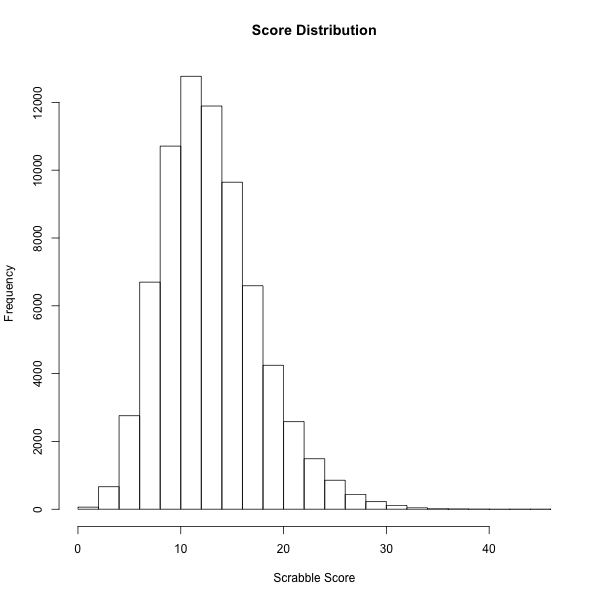
\includegraphics[width=0.4 \linewidth,trim={0 0 0 0}, clip=true]{scrabble_hist.png}

\caption{Histogram of scrabble scores}

\label{fig:hist}

\end{figure}

\item There are \textbf{120} words with reverse complements in the database. These are:\\
A AL ARIZ AS B BIRD C CI CL D E F FLO FM G GILL H HE HF HG HO HORN HZ I IN IO IR J K L LN LOU LR LT LYRA M MILO MN MO MR N ND NOV O OK OORT ORLY OZ P PL POLK Q R RH RN RX S SI T U UR V W WM X Y YB Z ZIBO ZN ZOLA ASP BEVY BID BIG BOIL BOORISH BOORS BY ELM GIRT GO GRID GRIT HI HILLY HOOFS HOVELS HULLS IF KHZ LO LORN LS MA MI MILD MILK MILS NU OX PORN RS SH SHRILLY TRIG TRY TS US VELD VOLE VS WILD WIRY WIZARD WORD WORN WOVE WRIT WRY

\item From the list of [F A L U Y P L N I], we can construct \textbf{39} words at least 4 letters long and containing the letter 'A' that are in the database. These are:\\
ALLY AINU FALL FAUN FAIL FAIN FLAY FLAP FLAN FLAIL FULANI FINAL FINALLY LAIN LULA LUNA LILA LINA ULNA YALU YUAN PALL PAUL PAULI PAIL PAILFUL PAIN PAINFUL PAINFULLY PLAY PLAYFUL PLAN PLAIN PLAINLY PIAF PILAF PILAU NAIL INLAY

\end{enumerate}

\section{Examination marking}

The filled-out table of student results is given in table \ref{tab:score}.

\begin{table}[h]
\centering
\begin{tabular}{ |c|c|c|c|}
\hline
student & score & grade & rank \\
\hline
1 & 19&B &6 \\
2 & 24&A & 2\\
3 & 14& D& 10\\
4 & 17& C& 8\\
5 & 20& B& 5\\
6 & 23& A& 3\\
7 & 29& A& 1\\
8 & 7& F& 12\\
9 & 22&A & 4\\
10 &17 & C& 8\\
11 & 9& F& 11\\
12 & 18& C& 7\\
\hline

\end{tabular}
\caption{Student examination results}
\label{tab:score}
\end{table}


To test for students cheating, we define a pairwise penalty function between two students which quantifies how similar their answers are. If we denote the average proportion of correctly answered questions p, the probability of two students both answering a question correctly given both students attempting the question and no cheating occurring is\\\\
$P(c,c | ans, no\_cheat) = p^2$\\\\
On the other hand, the probability that they both give the same incorrect answer is\\\\
$P(i,i | ans, no\_cheat) = (\dfrac{1-p}{4})^2$\\\\
Since probabilities are multiplicative, their logs are additive and we can therefore define a probabilistic similarity score based on log likelihoods which we denote S\\\\
 $S(a,b) = -N(c,c)*log_{10}(p^2) - N(i,i)*log_{10}((\dfrac{1-p}{4})^2)$\\\\
Where $N(c,c)$ and $N(i,i)$ are the number of identical correct and incorrect answers respectively between students a and b. In the present case, $p = 0.608$ giving $-log_{10}(p^2) = 0.43$ and $-log_{10}((\dfrac{1-p}{4})^2)=2.02$. A funtion has been written that will automatically check if two students have similar results based on this similarity measure (see code).

It is hard to predict what the similarity distribution would be in the absence of cheating, as it will be biased towards more similarity if some questions are easier than others, leading to a higher proportion of students picking similar questions than expected by random chance, or if some wrong options are more likely to be picked than others.

However, we can visualize the distribution of all 66 pairwise similarity scores (figure \ref{fig:cheat_hist}). If we assume that the majority of students do not cheat, we would expect pairs of cheating students to give rise to outliers in the distribution. We can also visualize this in two dimensions by plotting a heatmap of similarity scores. 

\begin{figure}[h]
\centering

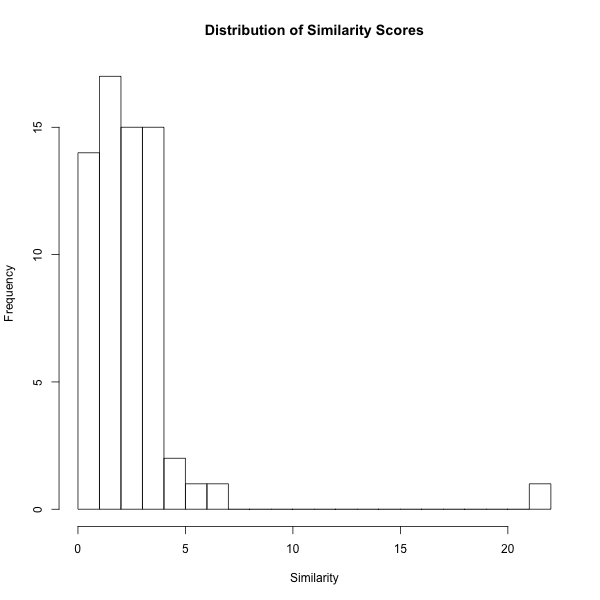
\includegraphics[width=0.4 \linewidth,trim={0 0 0 0}, clip=true]{cheat_hist.png}
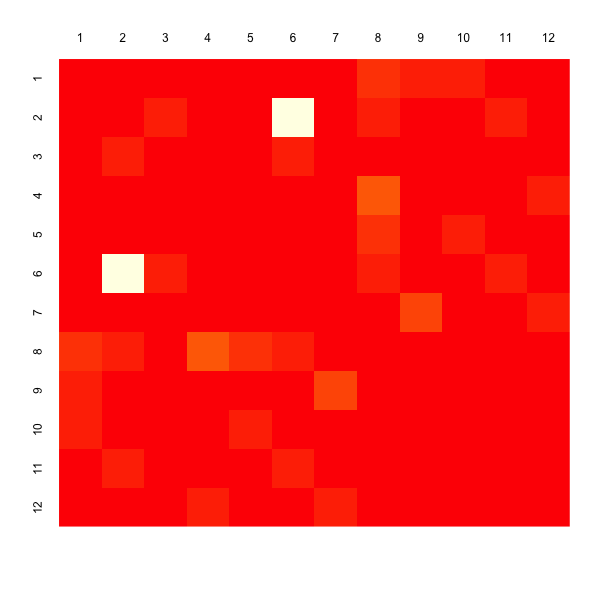
\includegraphics[width=0.4 \linewidth,trim={0 0 0 0}, clip=true]{cheat_heat.png}

\caption{Histogram (left) and heatmap (right) of similarity scores}
\label{fig:cheat_hist}


\end{figure}

We clearly see that one pair of students is a significant outlier, and that this pair consists of students 2 and 6. To make this slightly more quantitative, we can rank the similarity scores with the top 5 pairs given in table \ref{tab:sim}. The number of standard deviations each pair is from the mean of all \textit{other} similarity scores is also given, since we may assume that cheating scores will deviate from the non-cheating distribution.

\begin{table}[h]
\centering
\begin{tabular}{ |c|c|c|}
\hline
Pair & Similarity & Standard Deviations \\
\hline
(2,6) & 21.2&14.2  \\
(4,8) & 6.5&1.5 \\
(7,9) & 5.5& 1.1\\
(1,8) & 4.9& 0.9\\
(5,8) & 4.5& 0.8\\
\hline

\end{tabular}
\caption{Table of similarity scores}
\label{tab:sim}
\end{table}

Again we see the pair (2, 6) as a significant outlier, whereas the other high-scoring pairs are not far enough from the mean to justify accusations of cheating. It is worth noting that this analysis is somewhat confounded by the (2,6) pair being a far outlier and thus bringing up the standard deviation of the set of similarity scores where it is not excluded, leading to relatively smaller deviations for the remaining pairs.

After concluding that the responses of students 2 and 6 are suspiciously similar, we can check the actual data and see that they answered 27 of the same questions and gave the same answer to every question they both answered, even though 6 of these were incorrect. We thus conclude that students 2 and 6 cheated, although it is not clear if there was a directionality to the cheating.

We can now remove the S(2,6) from our list of scores and rerun the analysis to see if any other pairs are suspiciously far off the distribution mean (table \ref{tab:sim2}).

\begin{table}[h]
\centering
\begin{tabular}{ |c|c|c|}
\hline
Pair & Similarity & Standard Deviations \\
\hline
(4,8) & 6.5&3.6 \\
(7,9) & 5.5& 2.6\\
(1,8) & 4.9& 2.1\\
(5,8) & 4.5& 1.8\\
\hline

\end{tabular}
\caption{Table of similarity scores after removing S(2,6)}
\label{tab:sim2}
\end{table}

These scores do not seem particularly suspicious, although if we assume scores to be normally distributed, there is only a 0.02\% chance of a score being 3.6 standard deviations from the mean which might be considered significant even after correcting for 65 comparisons.

This has been automatized further in the function catch\_cheat where, given a Bonferroni-corrected cutoff of e.g. 0.01, pairs of potentially cheating students are iteratively flagged and removed until there are none exceeding this threshold (with a threshold of 0.01, only the pair (2,6) are flagged as cheating).

\newpage

\section{Appendix}

\lstinputlisting[language=R]{code_sp.R}




\end{document}